% ***********************************************************
% ******************* PHYSICS HEADER ************************
% ***********************************************************
% Version 2
\documentclass[11pt]{article} 
\usepackage{amsmath} % AMS Math Package
\usepackage{amsthm} % Theorem Formatting
\usepackage{amssymb}	% Math symbols such as \mathbb
\usepackage{graphicx} % Allows for eps images
\usepackage{multicol} % Allows for multiple columns
\usepackage[dvips]{geometry}
 % Sets margins and page size
\pagestyle{empty} % Removes page numbers
\makeatletter % Need for anything that contains an @ command 
\renewcommand{\maketitle} % Redefine maketitle to conserve space
{ \begingroup \vskip 10pt \begin{center} \large {\bf \@title}
	\vskip 10pt \large \@author \hskip 20pt \@date \end{center}
  \vskip 10pt \endgroup \setcounter{footnote}{0} }
\makeatother % End of region containing @ commands
\renewcommand{\labelenumi}{(\alph{enumi})} % Use letters for enumerate
% \DeclareMathOperator{\Sample}{Sample}
\let\vaccent=\v % rename builtin command \v{} to \vaccent{}
\renewcommand{\v}[1]{\ensuremath{\mathbf{#1}}} % for vectors
\newcommand{\gv}[1]{\ensuremath{\mbox{\boldmath$ #1 $}}} 
% for vectors of Greek letters
\newcommand{\uv}[1]{\ensuremath{\mathbf{\hat{#1}}}} % for unit vector
\newcommand{\abs}[1]{\left| #1 \right|} % for absolute value
\newcommand{\avg}[1]{\left< #1 \right>} % for average
\let\underdot=\d % rename builtin command \d{} to \underdot{}
\renewcommand{\d}[2]{\frac{d #1}{d #2}} % for derivatives
\newcommand{\dd}[2]{\frac{d^2 #1}{d #2^2}} % for double derivatives
\newcommand{\pd}[2]{\frac{\partial #1}{\partial #2}} 
% for partial derivatives
\newcommand{\pdd}[2]{\frac{\partial^2 #1}{\partial #2^2}} 
% for double partial derivatives
\newcommand{\pdc}[3]{\left( \frac{\partial #1}{\partial #2}
 \right)_{#3}} % for thermodynamic partial derivatives
\newcommand{\ket}[1]{\left| #1 \right>} % for Dirac bras
\newcommand{\bra}[1]{\left< #1 \right|} % for Dirac kets
\newcommand{\braket}[2]{\left< #1 \vphantom{#2} \right|
 \left. #2 \vphantom{#1} \right>} % for Dirac brackets
\newcommand{\matrixel}[3]{\left< #1 \vphantom{#2#3} \right|
 #2 \left| #3 \vphantom{#1#2} \right>} % for Dirac matrix elements
\newcommand{\grad}[1]{\gv{\nabla} #1} % for gradient
\let\divsymb=\div % rename builtin command \div to \divsymb
\renewcommand{\div}[1]{\gv{\nabla} \cdot #1} % for divergence
\newcommand{\curl}[1]{\gv{\nabla} \times #1} % for curl
\let\baraccent=\= % rename builtin command \= to \baraccent
\renewcommand{\=}[1]{\stackrel{#1}{=}} % for putting numbers above =
\newtheorem{prop}{Proposition}
\newtheorem{thm}{Theorem}[section]
\newtheorem{lem}[thm]{Lemma}
\theoremstyle{definition}
\newtheorem{dfn}{Definition}
\theoremstyle{remark}
\newtheorem*{rmk}{Remark}

% ***********************************************************
% ********************** END HEADER *************************
% ***********************************************************

%%% Local Variables:
%%% mode: latex
%%% TeX-Master: notes
%%% End:

\usepackage[utf8]{inputenc}
\usepackage{amsmath}
\usepackage{amssymb}
\usepackage{amsfonts}
\usepackage{amssymb}
\usepackage{float}
\usepackage{indentfirst}
\usepackage{vmargin}
\usepackage{indentfirst}
\usepackage{titling}
\usepackage{color} 
\usepackage{siunitx}
\usepackage{xspace}
\usepackage{graphicx}
\usepackage{enumitem}
\usepackage{array}
\usepackage[backend=biber,backref=true,style=unsrt,
style=numeric-comp,block=ragged,firstinits=true]{biblatex}
\addbibresource{ref-notes.bib}
\bibliography{ref-notes}
\graphicspath{{plot_synthesis/} {Feynman/}}

\newcommand{\mastersig}{\ensuremath{\Im{\widehat{\Sigma}^{A,B}(k,E)}}\xspace}
\newcommand{\chiqw}{\ensuremath{\Im{\chi}(q,\omega)}\xspace}

\providecommand{\norm}[1]{\lVert#1\rVert}

\newcommand{\subtitle}[1]{%
  \posttitle{%
    \par\end{center}
    \begin{center}\large#1\end{center}
    \vskip0.5em}%
}

\title{F9800 Condensed Matter Physics II}
\subtitle{Final Exam}
%\author{}
\date{Spring 2014}

\begin{document}

\maketitle

\setlength{\unitlength}{1cm}
%\advance\textwidth by 3cm
%\advance\hoffset by -1.5cm 
\advance\textheight by 1cm
\advance\voffset by -1.5cm
\setmarginsrb{3cm}{0.5cm}{1.5cm}{1cm}{1cm}{1cm}{1cm}{1cm}
%\setlength{\parindent}{0cm}%

\pagestyle{plain}

\vspace{2cm}

\textbf{Date:} \hspace{6cm} \textbf{Name:}

\vspace{1cm}

\section{Band structure}

\subsection{Introduction}

Figure~\ref{fig:bands} shows the diagram of energy versus wave vector, for
electrons in a 1D solid.

\begin{figure}[h]
  \centering
  \includegraphics[width=10cm]{Final_bands.pdf}
  \caption{Band structure of a 1D solid.\label{fig:bands}}
\end{figure}

\subsection{Questions}

\begin{enumerate}[label=(\roman*)]
\item If we note $n$ the density of electrons, and $p$ the density of
  holes, what assertion can you formulate about the value of the ratio
  $\dfrac{p}{n}$?
\item Can you infer from Fig.~\ref{fig:bands} if this material has an
  even or odd number of electrons per unit cell? Justify your answer.
\item Which is greater: the effective masses of the electron, or that
  of the hole? Derive approximate expressions for the effective masses
  in terms of quantities in the diagram.
\end{enumerate}

\section{Donor states in Ge}

\subsection{Introduction}

The conduction band of Germanium exhibits four equivalent minima at
the L points of the Brillouin zone. The (orthonormal) electronic state
vectors in such directions are designated by the following symbols:

\begin{itemize}
\item $\ket{a}$ for the minimum in direction $[1\bar{1}\bar{1}]$
\item $\ket{b}$ for the minimum in direction $[\bar{1}1\bar{1}]$
\item $\ket{c}$ for the minimum in direction $[111]$
\item $\ket{d}$ for the minimum in direction $[\bar{1}\bar{1}1]$
\end{itemize}

\begin{figure}[h]
  \centering
  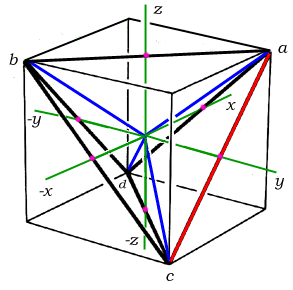
\includegraphics[width=7cm]{xyzcube.png}
  \caption{Regular tetrahedron with Ge atoms on the a, b, c,
    and d sites. A donor atom is located in the middle of the tetrahedron.\label{fig:tetra}}
\end{figure}

A donor atom is located at the center of a regular tetrahedron as
indicated in Fig~\ref{fig:tetra}. As a reminder, the group of
symmetries of the regular tetrahedraon is $T_d$, of order 24, with elements:

\begin{itemize}
\item $E$ (identity)
\item 8 rotations  $C_3$ about the diagonals of a cube.
\item 3 rotations $C_2$ about axes $x, y , z$.
\item 6 reflections $\sigma_d$ in planes containing one edge and the center of
  the tetrahedron (diagonal axes).
\item 6 improper rotations $S_4$ about axis $x, y , z$ (rotations
of angle $\pi/2$ followed by a reflection in a plane perpendicular to
the axis of rotation).
\end{itemize}

Its character table is the following:

\begin{center}
 \begin{tabular}{|| l | *{5}{c} ||} 
 \hline
   & E & 8$C_3$ & 3$C_2$ & 6$\sigma_d$ & 6$S_4$ \\ [0.5ex] 
 \hline\hline
 $A_1$ & 1 & 1 & 1 & 1 & 1 \\ 
 \hline
 $A_2$ & 1 & 1 & 1 & -1 & -1 \\ 
 \hline
 $E$ & 2 & -1 & 2 & 0 & 0 \\ 
 \hline
 $T_1$ & 3 & 0 & -1 & -1 & 1 \\ 
 \hline
 $T_2$ & 3 & 0 & -1 & 1 & -1 \\
 \hline
\end{tabular}
\end{center}

\subsection{Questions}

\begin{enumerate}[label=(\roman*)]
\item Apply one symmetry operation of each class of the $T_d$ group to
  the four dimensional vector $\begin{pmatrix}
\ket{a}\\ 
\ket{b}\\
\ket{c}\\
\ket{d}\\
\end{pmatrix}$
\item Using the previous result, establish the character table of the
  four-dimensional representation $R_4$ of the group $T_d$.
\item Using the character
  table of the $T_d$ group, decompose $R_4$ into its irreducible
  components. Such decomposition should be the result of an explicit
  calculation, i.e. the result should not only be established by inspection.
\item Verify that the following symmetrized combinations of state
  vectors are bases of the corresponding irreducible representations
  of the $T_d$ group:
  \begin {itemize}
  \item $A_1: \dfrac{\ket{a} + \ket{b} + \ket{c} + \ket{d}}{2}$
  \item $T_2: $ \begin{itemize}
    \item $\ket{pmpm} = \dfrac{\ket{a} - \ket{b} + \ket{c} -
        \ket{d}}{2}$
    \item $\ket{ppmm} = \dfrac{\ket{a} + \ket{b} - \ket{c} -
        \ket{d}}{2}$
    \item $\ket{pmmp} = \dfrac{\ket{a} - \ket{b} - \ket{c} +
        \ket{d}}{2}$
    \end{itemize}
  \end{itemize}
\end{enumerate}



%\section

\end{document}